% Options for packages loaded elsewhere
\PassOptionsToPackage{unicode}{hyperref}
\PassOptionsToPackage{hyphens}{url}
%
\documentclass[
]{article}
\usepackage{amsmath,amssymb}
\usepackage{lmodern}
\usepackage{iftex}
\ifPDFTeX
  \usepackage[T1]{fontenc}
  \usepackage[utf8]{inputenc}
  \usepackage{textcomp} % provide euro and other symbols
\else % if luatex or xetex
  \usepackage{unicode-math}
  \defaultfontfeatures{Scale=MatchLowercase}
  \defaultfontfeatures[\rmfamily]{Ligatures=TeX,Scale=1}
\fi
% Use upquote if available, for straight quotes in verbatim environments
\IfFileExists{upquote.sty}{\usepackage{upquote}}{}
\IfFileExists{microtype.sty}{% use microtype if available
  \usepackage[]{microtype}
  \UseMicrotypeSet[protrusion]{basicmath} % disable protrusion for tt fonts
}{}
\makeatletter
\@ifundefined{KOMAClassName}{% if non-KOMA class
  \IfFileExists{parskip.sty}{%
    \usepackage{parskip}
  }{% else
    \setlength{\parindent}{0pt}
    \setlength{\parskip}{6pt plus 2pt minus 1pt}}
}{% if KOMA class
  \KOMAoptions{parskip=half}}
\makeatother
\usepackage{xcolor}
\usepackage[left=1cm,right=1cm,top=2cm,bottom=2cm]{geometry}
\usepackage{color}
\usepackage{fancyvrb}
\newcommand{\VerbBar}{|}
\newcommand{\VERB}{\Verb[commandchars=\\\{\}]}
\DefineVerbatimEnvironment{Highlighting}{Verbatim}{commandchars=\\\{\}}
% Add ',fontsize=\small' for more characters per line
\usepackage{framed}
\definecolor{shadecolor}{RGB}{248,248,248}
\newenvironment{Shaded}{\begin{snugshade}}{\end{snugshade}}
\newcommand{\AlertTok}[1]{\textcolor[rgb]{0.94,0.16,0.16}{#1}}
\newcommand{\AnnotationTok}[1]{\textcolor[rgb]{0.56,0.35,0.01}{\textbf{\textit{#1}}}}
\newcommand{\AttributeTok}[1]{\textcolor[rgb]{0.77,0.63,0.00}{#1}}
\newcommand{\BaseNTok}[1]{\textcolor[rgb]{0.00,0.00,0.81}{#1}}
\newcommand{\BuiltInTok}[1]{#1}
\newcommand{\CharTok}[1]{\textcolor[rgb]{0.31,0.60,0.02}{#1}}
\newcommand{\CommentTok}[1]{\textcolor[rgb]{0.56,0.35,0.01}{\textit{#1}}}
\newcommand{\CommentVarTok}[1]{\textcolor[rgb]{0.56,0.35,0.01}{\textbf{\textit{#1}}}}
\newcommand{\ConstantTok}[1]{\textcolor[rgb]{0.00,0.00,0.00}{#1}}
\newcommand{\ControlFlowTok}[1]{\textcolor[rgb]{0.13,0.29,0.53}{\textbf{#1}}}
\newcommand{\DataTypeTok}[1]{\textcolor[rgb]{0.13,0.29,0.53}{#1}}
\newcommand{\DecValTok}[1]{\textcolor[rgb]{0.00,0.00,0.81}{#1}}
\newcommand{\DocumentationTok}[1]{\textcolor[rgb]{0.56,0.35,0.01}{\textbf{\textit{#1}}}}
\newcommand{\ErrorTok}[1]{\textcolor[rgb]{0.64,0.00,0.00}{\textbf{#1}}}
\newcommand{\ExtensionTok}[1]{#1}
\newcommand{\FloatTok}[1]{\textcolor[rgb]{0.00,0.00,0.81}{#1}}
\newcommand{\FunctionTok}[1]{\textcolor[rgb]{0.00,0.00,0.00}{#1}}
\newcommand{\ImportTok}[1]{#1}
\newcommand{\InformationTok}[1]{\textcolor[rgb]{0.56,0.35,0.01}{\textbf{\textit{#1}}}}
\newcommand{\KeywordTok}[1]{\textcolor[rgb]{0.13,0.29,0.53}{\textbf{#1}}}
\newcommand{\NormalTok}[1]{#1}
\newcommand{\OperatorTok}[1]{\textcolor[rgb]{0.81,0.36,0.00}{\textbf{#1}}}
\newcommand{\OtherTok}[1]{\textcolor[rgb]{0.56,0.35,0.01}{#1}}
\newcommand{\PreprocessorTok}[1]{\textcolor[rgb]{0.56,0.35,0.01}{\textit{#1}}}
\newcommand{\RegionMarkerTok}[1]{#1}
\newcommand{\SpecialCharTok}[1]{\textcolor[rgb]{0.00,0.00,0.00}{#1}}
\newcommand{\SpecialStringTok}[1]{\textcolor[rgb]{0.31,0.60,0.02}{#1}}
\newcommand{\StringTok}[1]{\textcolor[rgb]{0.31,0.60,0.02}{#1}}
\newcommand{\VariableTok}[1]{\textcolor[rgb]{0.00,0.00,0.00}{#1}}
\newcommand{\VerbatimStringTok}[1]{\textcolor[rgb]{0.31,0.60,0.02}{#1}}
\newcommand{\WarningTok}[1]{\textcolor[rgb]{0.56,0.35,0.01}{\textbf{\textit{#1}}}}
\usepackage{longtable,booktabs,array}
\usepackage{calc} % for calculating minipage widths
% Correct order of tables after \paragraph or \subparagraph
\usepackage{etoolbox}
\makeatletter
\patchcmd\longtable{\par}{\if@noskipsec\mbox{}\fi\par}{}{}
\makeatother
% Allow footnotes in longtable head/foot
\IfFileExists{footnotehyper.sty}{\usepackage{footnotehyper}}{\usepackage{footnote}}
\makesavenoteenv{longtable}
\usepackage{graphicx}
\makeatletter
\def\maxwidth{\ifdim\Gin@nat@width>\linewidth\linewidth\else\Gin@nat@width\fi}
\def\maxheight{\ifdim\Gin@nat@height>\textheight\textheight\else\Gin@nat@height\fi}
\makeatother
% Scale images if necessary, so that they will not overflow the page
% margins by default, and it is still possible to overwrite the defaults
% using explicit options in \includegraphics[width, height, ...]{}
\setkeys{Gin}{width=\maxwidth,height=\maxheight,keepaspectratio}
% Set default figure placement to htbp
\makeatletter
\def\fps@figure{htbp}
\makeatother
\setlength{\emergencystretch}{3em} % prevent overfull lines
\providecommand{\tightlist}{%
  \setlength{\itemsep}{0pt}\setlength{\parskip}{0pt}}
\setcounter{secnumdepth}{-\maxdimen} % remove section numbering
\usepackage{float}
\floatplacement{figure}{H}
\renewcommand{\contentsname}{Contents}
\usepackage{mdframed}
\definecolor{shadecolor}{gray}{.90}
\renewenvironment{Shaded}{\begin{mdframed}[ backgroundcolor=shadecolor, linecolor = shadecolor, leftmargin=\dimexpr\leftmargin-2pt\relax, innerleftmargin=1.6pt, innertopmargin=5pt, skipabove=10pt,skipbelow=3pt ]}{\end{mdframed}}
\usepackage{booktabs}
\usepackage{longtable}
\usepackage{array}
\usepackage{multirow}
\usepackage{wrapfig}
\usepackage{float}
\usepackage{colortbl}
\usepackage{pdflscape}
\usepackage{tabu}
\usepackage{threeparttable}
\usepackage{threeparttablex}
\usepackage[normalem]{ulem}
\usepackage{makecell}
\usepackage{xcolor}
\ifLuaTeX
  \usepackage{selnolig}  % disable illegal ligatures
\fi
\IfFileExists{bookmark.sty}{\usepackage{bookmark}}{\usepackage{hyperref}}
\IfFileExists{xurl.sty}{\usepackage{xurl}}{} % add URL line breaks if available
\urlstyle{same} % disable monospaced font for URLs
\hypersetup{
  pdftitle={Analysis of the age variable},
  pdfauthor={José Carlos Soares Junior},
  hidelinks,
  pdfcreator={LaTeX via pandoc}}

\title{Analysis of the age variable}
\author{José Carlos Soares Junior}
\date{2023}

\begin{document}
\maketitle

{
\setcounter{tocdepth}{3}
\tableofcontents
}
\newpage

\hypertarget{r-packages}{%
\section{R packages}\label{r-packages}}

\begin{Shaded}
\begin{Highlighting}[]
\CommentTok{\# Load packages}
\NormalTok{loadlibrary }\OtherTok{\textless{}{-}} \ControlFlowTok{function}\NormalTok{(x) \{}
  \ControlFlowTok{if}\NormalTok{ (}\SpecialCharTok{!}\FunctionTok{require}\NormalTok{(x, }\AttributeTok{character.only =} \ConstantTok{TRUE}\NormalTok{)) \{}
    \FunctionTok{install.packages}\NormalTok{(x, }\AttributeTok{dependencies =}\NormalTok{ T)}
  \ControlFlowTok{if}\NormalTok{ (}\SpecialCharTok{!}\FunctionTok{require}\NormalTok{(x, }\AttributeTok{character.only =} \ConstantTok{TRUE}\NormalTok{))}
  \FunctionTok{stop}\NormalTok{(}\StringTok{"Package not found"}\NormalTok{)}
\NormalTok{  \}}
\NormalTok{\}}

\NormalTok{packages }\OtherTok{\textless{}{-}} \FunctionTok{c}\NormalTok{(}
  \StringTok{"readr"}\NormalTok{,}
  \StringTok{"readxl"}\NormalTok{,}
  \StringTok{"janitor"}\NormalTok{,}
  \StringTok{"dplyr"}\NormalTok{,}
  \StringTok{"forcats"}\NormalTok{,}
  \StringTok{"stringr"}\NormalTok{,}
  \StringTok{"lubridate"}\NormalTok{,}
  \StringTok{"summarytools"}\NormalTok{,}
  \StringTok{"magrittr"}\NormalTok{,}
  \StringTok{"questionr"}\NormalTok{,}
  \StringTok{"knitr"}\NormalTok{,}
  \StringTok{"data.table"}\NormalTok{,}
  \StringTok{"writexl"}\NormalTok{,}
  \StringTok{"modelsummary"}\NormalTok{,}
  \StringTok{"abjData"}\NormalTok{,}
  \StringTok{"aweek"}\NormalTok{,}
  \StringTok{"ggplot2"}\NormalTok{,}
  \StringTok{"viridis"}
\NormalTok{)}
\FunctionTok{lapply}\NormalTok{(packages, loadlibrary)}

\CommentTok{\# Global changes for the summarytools packages}
\FunctionTok{st\_options}\NormalTok{(}\AttributeTok{freq.cumul =} \ConstantTok{FALSE}\NormalTok{,          }
           \AttributeTok{display.labels =} \ConstantTok{TRUE}\NormalTok{,}
           \AttributeTok{lang =} \StringTok{"pt"}\NormalTok{,}
           \AttributeTok{bootstrap.css =} \ConstantTok{FALSE}\NormalTok{,}
           \AttributeTok{plain.ascii =} \ConstantTok{FALSE}\NormalTok{,}
           \AttributeTok{dfSummary.silent =} \ConstantTok{TRUE}\NormalTok{,}
           \AttributeTok{footnote =} \ConstantTok{NA}\NormalTok{,}
           \AttributeTok{subtitle.emphasis =} \ConstantTok{FALSE}\NormalTok{,}
           \AttributeTok{headings =} \ConstantTok{FALSE}\NormalTok{)}
\FunctionTok{st\_css}\NormalTok{()}
\end{Highlighting}
\end{Shaded}

\newpage

\hypertarget{data-preparation}{%
\section{Data preparation}\label{data-preparation}}

\begin{Shaded}
\begin{Highlighting}[]
\DocumentationTok{\#\#\#\#\#\#\#\#\#\#\#\#\#\#\#\#\#\#\#\#\#\# Loading the data \#\#\#\#\#\#\#\#\#\#\#\#\#\#\#\#\#\#\#\#\#\#\#}
\NormalTok{data\_age }\OtherTok{\textless{}{-}} \FunctionTok{readRDS}\NormalTok{(}\StringTok{"data\_paper\_1000d.rds"}\NormalTok{)}
\end{Highlighting}
\end{Shaded}

\begin{Shaded}
\begin{Highlighting}[]
\DocumentationTok{\#\#\#\#\#\#\#\#\#\#\#\#\#\#\#\#\#\#\#\#\#\# age variable \#\#\#\#\#\#\#\#\#\#\#\#\#\#\#\#\#\#\#\#\#\#\#}

\DocumentationTok{\#\#\#\#\#\#\#\# First case \#\#\#\#\#\#\#\#}
\CommentTok{\# \textless{}= 30 days (1 month);}
\CommentTok{\# 31 days |{-} 180 days (between 1 and 6 months); }
\CommentTok{\# 181 days |{-} 365 days (between 6 and 12 months); }
\CommentTok{\# \textgreater{}= 366 days (more than 12 months).}

\NormalTok{data\_age1 }\OtherTok{\textless{}{-}}\NormalTok{ data\_age }\SpecialCharTok{\%\textgreater{}\%}
  \FunctionTok{mutate}\NormalTok{(}\AttributeTok{age\_months\_firstcase =} \FunctionTok{case\_when}\NormalTok{(}
\NormalTok{    idade\_dias }\SpecialCharTok{\textless{}=} \DecValTok{30} \SpecialCharTok{\textasciitilde{}} \StringTok{"1 month"}\NormalTok{,}
\NormalTok{    idade\_dias }\SpecialCharTok{\textgreater{}} \DecValTok{30} \SpecialCharTok{\&}\NormalTok{ idade\_dias }\SpecialCharTok{\textless{}=} \DecValTok{180} \SpecialCharTok{\textasciitilde{}} \StringTok{"between 1 and 6 months"}\NormalTok{,}
\NormalTok{    idade\_dias }\SpecialCharTok{\textgreater{}} \DecValTok{180} \SpecialCharTok{\&}\NormalTok{ idade\_dias }\SpecialCharTok{\textless{}=} \DecValTok{365} \SpecialCharTok{\textasciitilde{}} \StringTok{"between 6 and 12 months"}\NormalTok{,}
\NormalTok{    idade\_dias }\SpecialCharTok{\textgreater{}} \DecValTok{365} \SpecialCharTok{\textasciitilde{}} \StringTok{"more than 12 months"}\NormalTok{) }
\NormalTok{    )}

\DocumentationTok{\#\#\#\#\#\#\#\# Second case \#\#\#\#\#\#\#\#}
\CommentTok{\# \textless{}= 30 days (1 month); }
\CommentTok{\# 31 days |{-} 180 days (between 1 and 6 months); }
\CommentTok{\# 181 days |{-} 365 days (between 6 and 12 months); }
\CommentTok{\# 366 days |{-} 545 days (between 12 and 18 months);}
\CommentTok{\# \textgreater{}= 546 days (more than 18 months).}

\NormalTok{data\_age2 }\OtherTok{\textless{}{-}}\NormalTok{ data\_age1 }\SpecialCharTok{\%\textgreater{}\%}
  \FunctionTok{mutate}\NormalTok{(}\AttributeTok{age\_months\_secondcase =} \FunctionTok{case\_when}\NormalTok{(}
\NormalTok{    idade\_dias }\SpecialCharTok{\textless{}=} \DecValTok{30} \SpecialCharTok{\textasciitilde{}} \StringTok{"1 month"}\NormalTok{,}
\NormalTok{    idade\_dias }\SpecialCharTok{\textgreater{}} \DecValTok{30} \SpecialCharTok{\&}\NormalTok{ idade\_dias }\SpecialCharTok{\textless{}=} \DecValTok{180} \SpecialCharTok{\textasciitilde{}} \StringTok{"between 1 and 6 months"}\NormalTok{,}
\NormalTok{    idade\_dias }\SpecialCharTok{\textgreater{}} \DecValTok{180} \SpecialCharTok{\&}\NormalTok{ idade\_dias }\SpecialCharTok{\textless{}=} \DecValTok{365} \SpecialCharTok{\textasciitilde{}} \StringTok{"between 6 and 12 months"}\NormalTok{,}
\NormalTok{    idade\_dias }\SpecialCharTok{\textgreater{}} \DecValTok{365} \SpecialCharTok{\&}\NormalTok{ idade\_dias }\SpecialCharTok{\textless{}=} \DecValTok{545} \SpecialCharTok{\textasciitilde{}} \StringTok{"between 12 and 18 months"}\NormalTok{,}
\NormalTok{    idade\_dias }\SpecialCharTok{\textgreater{}} \DecValTok{545} \SpecialCharTok{\textasciitilde{}} \StringTok{"more than 18 months"}\NormalTok{) }
\NormalTok{    )}
\end{Highlighting}
\end{Shaded}

\hypertarget{quantitative-analysis}{%
\section{Quantitative analysis}\label{quantitative-analysis}}

\hypertarget{analysis-of-agedays}{%
\subsection{Analysis of age(days)}\label{analysis-of-agedays}}

\begin{Shaded}
\begin{Highlighting}[]
\FunctionTok{ggplot}\NormalTok{(data\_age2, }\FunctionTok{aes}\NormalTok{(}\AttributeTok{x =}\NormalTok{ idade\_dias)) }\SpecialCharTok{+} 
  \FunctionTok{geom\_histogram}\NormalTok{(}\FunctionTok{aes}\NormalTok{(}\AttributeTok{y =} \FunctionTok{after\_stat}\NormalTok{(density)), }
                 \AttributeTok{bins =} \DecValTok{125}\NormalTok{,}
                 \AttributeTok{colour =} \StringTok{"black"}\NormalTok{,}
                 \AttributeTok{fill =} \StringTok{"white"}\NormalTok{) }\SpecialCharTok{+}
  \FunctionTok{geom\_density}\NormalTok{(}\AttributeTok{alpha =}\NormalTok{ .}\DecValTok{2}\NormalTok{, }\AttributeTok{fill =} \StringTok{"\#FF6666"}\NormalTok{) }\SpecialCharTok{+}
  \FunctionTok{labs}\NormalTok{(}\AttributeTok{x =} \StringTok{"}\SpecialCharTok{\textbackslash{}n}\StringTok{Age(days)"}\NormalTok{,}
       \AttributeTok{y =} \StringTok{"Density}\SpecialCharTok{\textbackslash{}n}\StringTok{"}\NormalTok{,}
       \AttributeTok{title =} \StringTok{"Histogram of age(days)"}\NormalTok{)}
\end{Highlighting}
\end{Shaded}

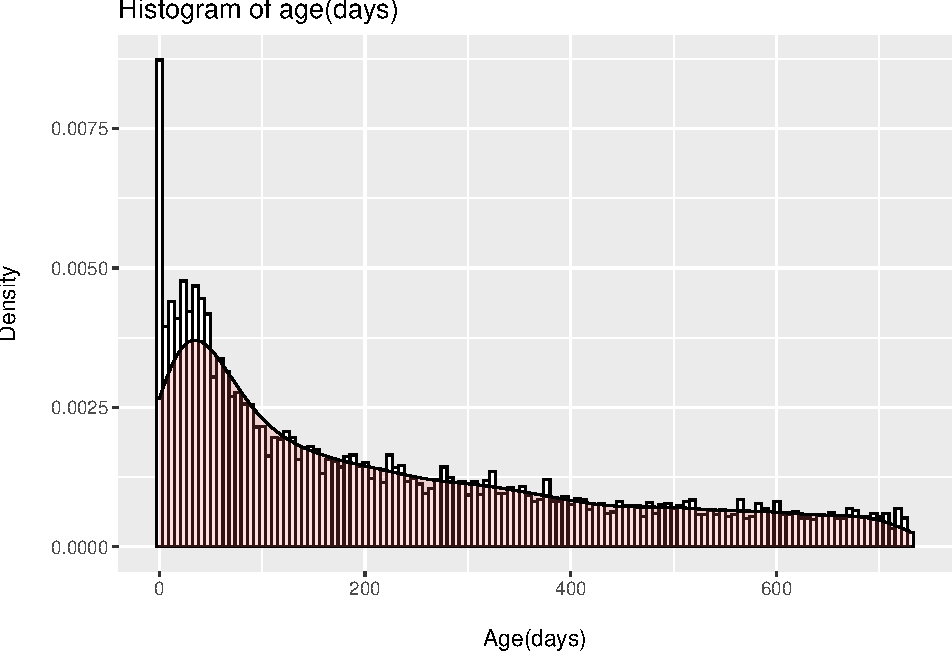
\includegraphics{age_analysis_files/figure-latex/unnamed-chunk-3-1.pdf}

\textbf{Figure 1:} Histogram of age in unit of days (bars) and density
(curve with red area).

\begin{Shaded}
\begin{Highlighting}[]
\NormalTok{data\_age2}\SpecialCharTok{$}\NormalTok{variants }\OtherTok{\textless{}{-}} \FunctionTok{factor}\NormalTok{(data\_age2}\SpecialCharTok{$}\NormalTok{variants, }
                             \AttributeTok{levels =} \FunctionTok{c}\NormalTok{(}\StringTok{"original"}\NormalTok{,}
                                        \StringTok{"gamma"}\NormalTok{,}
                                        \StringTok{"delta"}\NormalTok{,}
                                        \StringTok{"omicron"}\NormalTok{)}
\NormalTok{                             )}

\NormalTok{data\_age2 }\SpecialCharTok{\%\textgreater{}\%} 
  \FunctionTok{ggplot}\NormalTok{(}\FunctionTok{aes}\NormalTok{(}\AttributeTok{x =}\NormalTok{ variants,}
             \AttributeTok{y =}\NormalTok{ idade\_dias,}
             \AttributeTok{fill =}\NormalTok{ variants)) }\SpecialCharTok{+}
  \FunctionTok{geom\_boxplot}\NormalTok{() }\SpecialCharTok{+}
  \FunctionTok{xlab}\NormalTok{(}\StringTok{"}\SpecialCharTok{\textbackslash{}n}\StringTok{Variants"}\NormalTok{) }\SpecialCharTok{+}
  \FunctionTok{ylab}\NormalTok{(}\StringTok{"Age(Days)}\SpecialCharTok{\textbackslash{}n}\StringTok{"}\NormalTok{) }\SpecialCharTok{+}
  \FunctionTok{theme}\NormalTok{(}\AttributeTok{legend.position =} \StringTok{"none"}\NormalTok{)}
\end{Highlighting}
\end{Shaded}

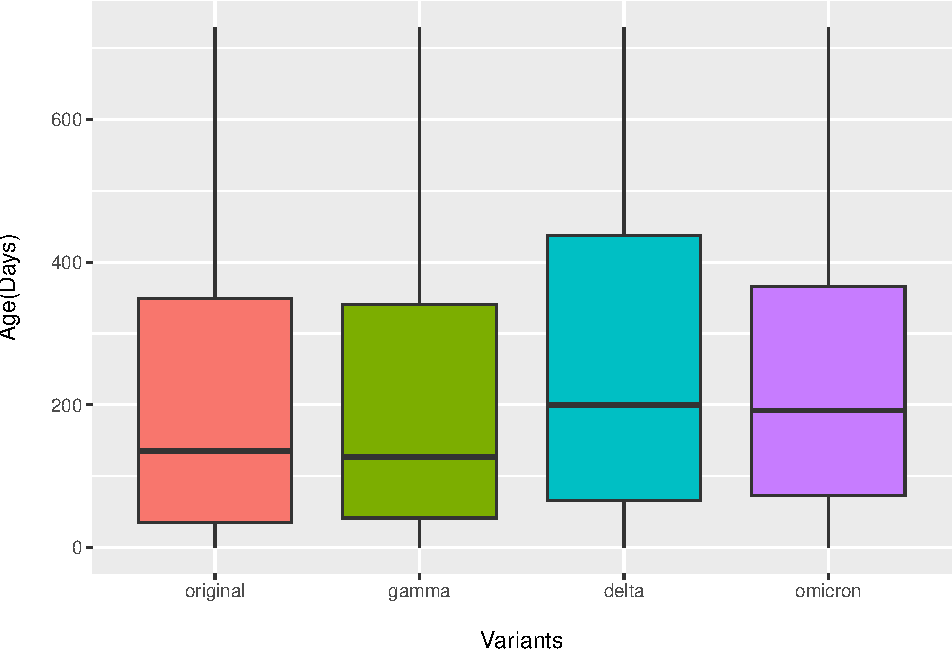
\includegraphics{age_analysis_files/figure-latex/unnamed-chunk-4-1.pdf}

\textbf{Figure 2:} Boxplot of variants by age in a unit of days.

\begin{Shaded}
\begin{Highlighting}[]
\CommentTok{\# Summary measurement functions}
\NormalTok{media }\OtherTok{\textless{}{-}} \ControlFlowTok{function}\NormalTok{(x) }
  \FunctionTok{mean}\NormalTok{(x, }\AttributeTok{na.rm =} \ConstantTok{TRUE}\NormalTok{)}
\NormalTok{mediana }\OtherTok{\textless{}{-}} \ControlFlowTok{function}\NormalTok{(x)}
  \FunctionTok{median}\NormalTok{(x, }\AttributeTok{na.rm =} \ConstantTok{TRUE}\NormalTok{)}
\NormalTok{DP }\OtherTok{\textless{}{-}} \ControlFlowTok{function}\NormalTok{(x)}
  \FunctionTok{sd}\NormalTok{(x, }\AttributeTok{na.rm =} \ConstantTok{TRUE}\NormalTok{)}
\NormalTok{minimo }\OtherTok{\textless{}{-}} \ControlFlowTok{function}\NormalTok{(x)}
\NormalTok{  base}\SpecialCharTok{::}\FunctionTok{min}\NormalTok{(x, }\AttributeTok{na.rm =} \ConstantTok{TRUE}\NormalTok{)}
\NormalTok{maximo }\OtherTok{\textless{}{-}} \ControlFlowTok{function}\NormalTok{(x) }
\NormalTok{  base}\SpecialCharTok{::}\FunctionTok{max}\NormalTok{(x, }\AttributeTok{na.rm =} \ConstantTok{TRUE}\NormalTok{)}
\NormalTok{q25 }\OtherTok{\textless{}{-}} \ControlFlowTok{function}\NormalTok{(x) }
\NormalTok{  stats}\SpecialCharTok{::}\FunctionTok{quantile}\NormalTok{(x, }\AttributeTok{p =} \FloatTok{0.25}\NormalTok{, }\AttributeTok{na.rm =} \ConstantTok{TRUE}\NormalTok{)}
\NormalTok{q75 }\OtherTok{\textless{}{-}} \ControlFlowTok{function}\NormalTok{(x)}
\NormalTok{  stats}\SpecialCharTok{::}\FunctionTok{quantile}\NormalTok{(x, }\AttributeTok{p =} \FloatTok{0.75}\NormalTok{, }\AttributeTok{na.rm =} \ConstantTok{TRUE}\NormalTok{)}
\NormalTok{IQR }\OtherTok{\textless{}{-}} \ControlFlowTok{function}\NormalTok{(x) }
  \FunctionTok{round}\NormalTok{(}\FunctionTok{q75}\NormalTok{(x) }\SpecialCharTok{{-}} \FunctionTok{q25}\NormalTok{(x), }\DecValTok{2}\NormalTok{)}
\NormalTok{n }\OtherTok{\textless{}{-}} \ControlFlowTok{function}\NormalTok{(x) }
  \FunctionTok{sum}\NormalTok{(}\SpecialCharTok{!}\FunctionTok{is.na}\NormalTok{(x))}
\end{Highlighting}
\end{Shaded}

\newpage

\begin{Shaded}
\begin{Highlighting}[]
\FunctionTok{datasummary}\NormalTok{(variants }\SpecialCharTok{\textasciitilde{}}\NormalTok{ idade\_dias}\SpecialCharTok{*}\NormalTok{(n }\SpecialCharTok{+}\NormalTok{ media }\SpecialCharTok{+}\NormalTok{ DP }\SpecialCharTok{+}\NormalTok{ mediana }\SpecialCharTok{+}\NormalTok{ minimo }\SpecialCharTok{+}
\NormalTok{                                   maximo }\SpecialCharTok{+}\NormalTok{ q25 }\SpecialCharTok{+}\NormalTok{ q75 }\SpecialCharTok{+}\NormalTok{ IQR), }
            \AttributeTok{data =}\NormalTok{ data\_age2, }\AttributeTok{output =} \StringTok{\textquotesingle{}markdown\textquotesingle{}}\NormalTok{)}
\end{Highlighting}
\end{Shaded}

\begin{longtable}[]{@{}
  >{\raggedright\arraybackslash}p{(\columnwidth - 18\tabcolsep) * \real{0.1286}}
  >{\raggedleft\arraybackslash}p{(\columnwidth - 18\tabcolsep) * \real{0.0714}}
  >{\raggedleft\arraybackslash}p{(\columnwidth - 18\tabcolsep) * \real{0.1000}}
  >{\raggedleft\arraybackslash}p{(\columnwidth - 18\tabcolsep) * \real{0.1000}}
  >{\raggedleft\arraybackslash}p{(\columnwidth - 18\tabcolsep) * \real{0.1143}}
  >{\raggedleft\arraybackslash}p{(\columnwidth - 18\tabcolsep) * \real{0.1000}}
  >{\raggedleft\arraybackslash}p{(\columnwidth - 18\tabcolsep) * \real{0.1000}}
  >{\raggedleft\arraybackslash}p{(\columnwidth - 18\tabcolsep) * \real{0.0857}}
  >{\raggedleft\arraybackslash}p{(\columnwidth - 18\tabcolsep) * \real{0.1000}}
  >{\raggedleft\arraybackslash}p{(\columnwidth - 18\tabcolsep) * \real{0.1000}}@{}}
\toprule()
\begin{minipage}[b]{\linewidth}\raggedright
variants
\end{minipage} & \begin{minipage}[b]{\linewidth}\raggedleft
n
\end{minipage} & \begin{minipage}[b]{\linewidth}\raggedleft
media
\end{minipage} & \begin{minipage}[b]{\linewidth}\raggedleft
DP
\end{minipage} & \begin{minipage}[b]{\linewidth}\raggedleft
mediana
\end{minipage} & \begin{minipage}[b]{\linewidth}\raggedleft
minimo
\end{minipage} & \begin{minipage}[b]{\linewidth}\raggedleft
maximo
\end{minipage} & \begin{minipage}[b]{\linewidth}\raggedleft
q25
\end{minipage} & \begin{minipage}[b]{\linewidth}\raggedleft
q75
\end{minipage} & \begin{minipage}[b]{\linewidth}\raggedleft
IQR
\end{minipage} \\
\midrule()
\endhead
original & 3706 & 210.63 & 207.17 & 135.00 & 0.00 & 730.00 & 35.00 &
348.75 & 313.75 \\
gamma & 2941 & 208.77 & 204.84 & 127.00 & 0.00 & 730.00 & 41.00 & 341.00
& 300.00 \\
delta & 795 & 259.04 & 215.66 & 200.00 & 0.00 & 729.00 & 66.00 & 437.00
& 371.00 \\
omicron & 3711 & 242.08 & 196.30 & 192.00 & 0.00 & 730.00 & 73.00 &
366.00 & 293.00 \\
\bottomrule()
\end{longtable}

\textbf{Table 1:} Descriptive metrics of age (days) by variants.

\hypertarget{analysis-of-agemonths}{%
\subsection{Analysis of age(months)}\label{analysis-of-agemonths}}

\begin{Shaded}
\begin{Highlighting}[]
\FunctionTok{ggplot}\NormalTok{(data\_age2, }\FunctionTok{aes}\NormalTok{(}\AttributeTok{x =}\NormalTok{ age\_month)) }\SpecialCharTok{+} 
  \FunctionTok{geom\_histogram}\NormalTok{(}\FunctionTok{aes}\NormalTok{(}\AttributeTok{y =} \FunctionTok{after\_stat}\NormalTok{(density)), }
                 \AttributeTok{bins =} \DecValTok{24}\NormalTok{,}
                 \AttributeTok{colour =} \StringTok{"black"}\NormalTok{,}
                 \AttributeTok{fill =} \StringTok{"white"}\NormalTok{) }\SpecialCharTok{+}
  \FunctionTok{geom\_density}\NormalTok{(}\AttributeTok{alpha =}\NormalTok{ .}\DecValTok{2}\NormalTok{, }\AttributeTok{fill =} \StringTok{"\#FF6666"}\NormalTok{) }\SpecialCharTok{+}
  \FunctionTok{labs}\NormalTok{(}\AttributeTok{x =} \StringTok{"}\SpecialCharTok{\textbackslash{}n}\StringTok{Age(month)"}\NormalTok{,}
       \AttributeTok{y =} \StringTok{"Density}\SpecialCharTok{\textbackslash{}n}\StringTok{"}\NormalTok{,}
       \AttributeTok{title =} \StringTok{"Histogram of age(month)"}\NormalTok{)}
\end{Highlighting}
\end{Shaded}

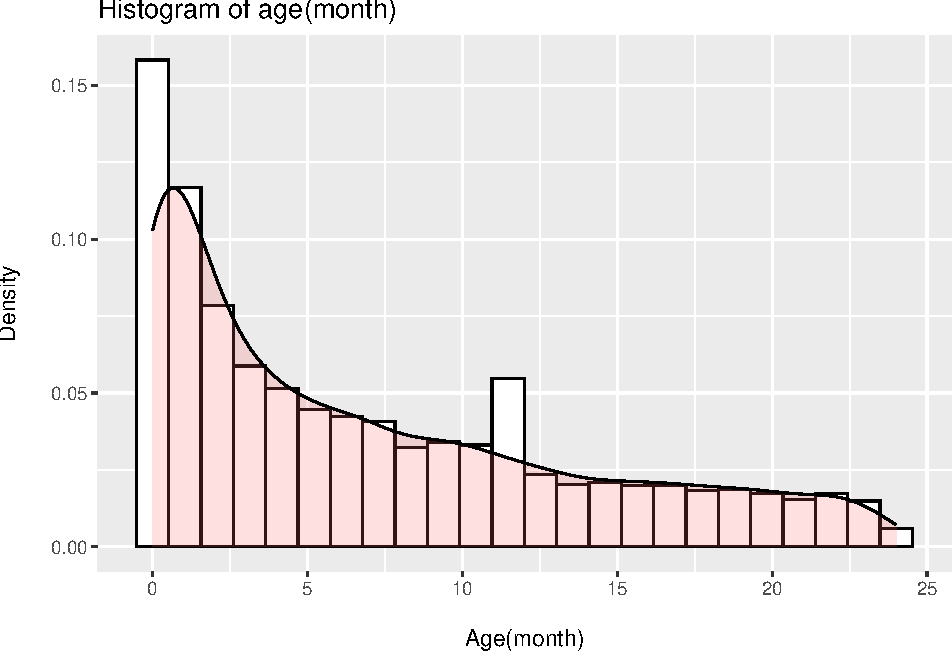
\includegraphics{age_analysis_files/figure-latex/unnamed-chunk-7-1.pdf}

\textbf{Figure 3:} Histogram of age in unit of months (bars) and density
(curve with red area).

\begin{Shaded}
\begin{Highlighting}[]
\NormalTok{data\_age2 }\SpecialCharTok{\%\textgreater{}\%} 
  \FunctionTok{ggplot}\NormalTok{(}\FunctionTok{aes}\NormalTok{(}\AttributeTok{x =}\NormalTok{ variants,}
             \AttributeTok{y =}\NormalTok{ age\_month,}
             \AttributeTok{fill =}\NormalTok{ variants)) }\SpecialCharTok{+}
  \FunctionTok{geom\_boxplot}\NormalTok{() }\SpecialCharTok{+}
  \FunctionTok{xlab}\NormalTok{(}\StringTok{"}\SpecialCharTok{\textbackslash{}n}\StringTok{Variants"}\NormalTok{) }\SpecialCharTok{+}
  \FunctionTok{ylab}\NormalTok{(}\StringTok{"Age(month)}\SpecialCharTok{\textbackslash{}n}\StringTok{"}\NormalTok{) }\SpecialCharTok{+}
  \FunctionTok{theme}\NormalTok{(}\AttributeTok{legend.position =} \StringTok{"none"}\NormalTok{)}
\end{Highlighting}
\end{Shaded}

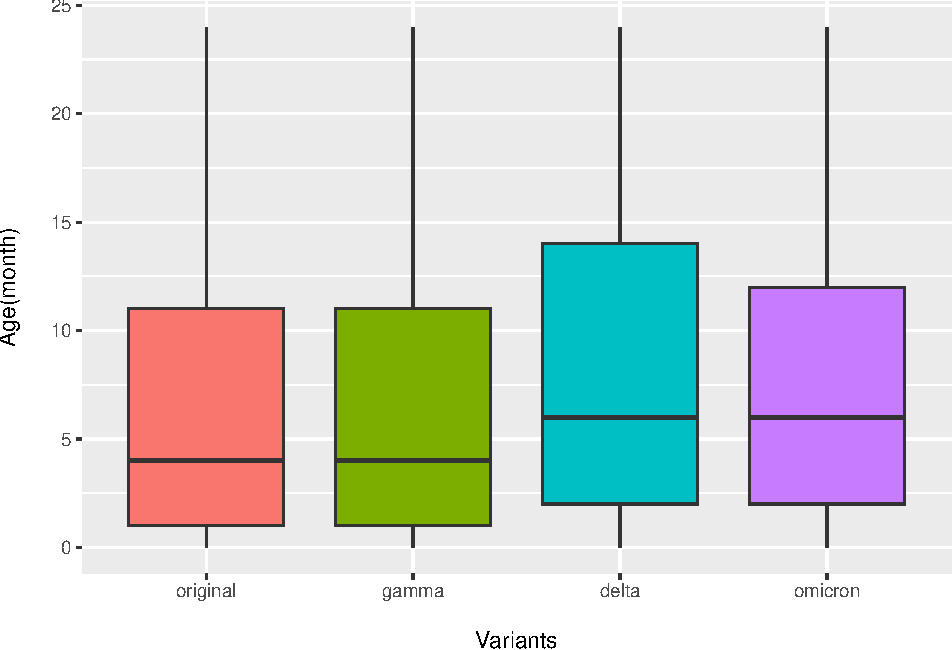
\includegraphics{age_analysis_files/figure-latex/unnamed-chunk-8-1.pdf}

\textbf{Figure 4:} Boxplot of variants by age in a unit of months.

\begin{Shaded}
\begin{Highlighting}[]
\FunctionTok{datasummary}\NormalTok{(variants }\SpecialCharTok{\textasciitilde{}}\NormalTok{ age\_month}\SpecialCharTok{*}\NormalTok{(n }\SpecialCharTok{+}\NormalTok{ media }\SpecialCharTok{+}\NormalTok{ DP }\SpecialCharTok{+}\NormalTok{ mediana }\SpecialCharTok{+}\NormalTok{ minimo }\SpecialCharTok{+}
\NormalTok{                                   maximo }\SpecialCharTok{+}\NormalTok{ q25 }\SpecialCharTok{+}\NormalTok{ q75 }\SpecialCharTok{+}\NormalTok{ IQR), }
            \AttributeTok{data =}\NormalTok{ data\_age2, }\AttributeTok{output =} \StringTok{\textquotesingle{}markdown\textquotesingle{}}\NormalTok{)}
\end{Highlighting}
\end{Shaded}

\begin{longtable}[]{@{}
  >{\raggedright\arraybackslash}p{(\columnwidth - 18\tabcolsep) * \real{0.1406}}
  >{\raggedleft\arraybackslash}p{(\columnwidth - 18\tabcolsep) * \real{0.0781}}
  >{\raggedleft\arraybackslash}p{(\columnwidth - 18\tabcolsep) * \real{0.0938}}
  >{\raggedleft\arraybackslash}p{(\columnwidth - 18\tabcolsep) * \real{0.0781}}
  >{\raggedleft\arraybackslash}p{(\columnwidth - 18\tabcolsep) * \real{0.1250}}
  >{\raggedleft\arraybackslash}p{(\columnwidth - 18\tabcolsep) * \real{0.1094}}
  >{\raggedleft\arraybackslash}p{(\columnwidth - 18\tabcolsep) * \real{0.1094}}
  >{\raggedleft\arraybackslash}p{(\columnwidth - 18\tabcolsep) * \real{0.0781}}
  >{\raggedleft\arraybackslash}p{(\columnwidth - 18\tabcolsep) * \real{0.0938}}
  >{\raggedleft\arraybackslash}p{(\columnwidth - 18\tabcolsep) * \real{0.0938}}@{}}
\toprule()
\begin{minipage}[b]{\linewidth}\raggedright
variants
\end{minipage} & \begin{minipage}[b]{\linewidth}\raggedleft
n
\end{minipage} & \begin{minipage}[b]{\linewidth}\raggedleft
media
\end{minipage} & \begin{minipage}[b]{\linewidth}\raggedleft
DP
\end{minipage} & \begin{minipage}[b]{\linewidth}\raggedleft
mediana
\end{minipage} & \begin{minipage}[b]{\linewidth}\raggedleft
minimo
\end{minipage} & \begin{minipage}[b]{\linewidth}\raggedleft
maximo
\end{minipage} & \begin{minipage}[b]{\linewidth}\raggedleft
q25
\end{minipage} & \begin{minipage}[b]{\linewidth}\raggedleft
q75
\end{minipage} & \begin{minipage}[b]{\linewidth}\raggedleft
IQR
\end{minipage} \\
\midrule()
\endhead
original & 3706 & 6.59 & 6.87 & 4.00 & 0.00 & 24.00 & 1.00 & 11.00 &
10.00 \\
gamma & 2941 & 6.51 & 6.80 & 4.00 & 0.00 & 24.00 & 1.00 & 11.00 &
10.00 \\
delta & 795 & 8.18 & 7.18 & 6.00 & 0.00 & 24.00 & 2.00 & 14.00 &
12.00 \\
omicron & 3711 & 7.59 & 6.54 & 6.00 & 0.00 & 24.00 & 2.00 & 12.00 &
10.00 \\
\bottomrule()
\end{longtable}

\textbf{Table 2:} Descriptive metrics of age (months) by variants.

\newpage

\hypertarget{grouped-age}{%
\section{Grouped age}\label{grouped-age}}

\hypertarget{first-case}{%
\subsection{First case}\label{first-case}}

\begin{Shaded}
\begin{Highlighting}[]
\DocumentationTok{\#\#\#\#\#\#\#\# First case \#\#\#\#\#\#\#\#}
\NormalTok{data\_age2}\SpecialCharTok{$}\NormalTok{age\_months\_firstcase }\OtherTok{\textless{}{-}} 
  \FunctionTok{as.factor}\NormalTok{(data\_age2}\SpecialCharTok{$}\NormalTok{age\_months\_firstcase)}

\NormalTok{summarytools}\SpecialCharTok{::}\FunctionTok{ctable}\NormalTok{(}
\NormalTok{        data\_age2}\SpecialCharTok{$}\NormalTok{age\_months\_firstcase,}
\NormalTok{        data\_age2}\SpecialCharTok{$}\NormalTok{variants,}
        \AttributeTok{prop =} \StringTok{"c"}\NormalTok{,}
        \AttributeTok{headings =} \FunctionTok{st\_options}\NormalTok{(}\StringTok{"headings"}\NormalTok{),}
        \AttributeTok{display.labels =} \FunctionTok{st\_options}\NormalTok{(}\StringTok{"display.labels"}\NormalTok{),}
        \AttributeTok{useNA =} \StringTok{"ifany"}\NormalTok{,}
        \AttributeTok{OR =} \ConstantTok{TRUE}\NormalTok{,}
        \AttributeTok{chisq =} \ConstantTok{TRUE}
\NormalTok{      )}
\end{Highlighting}
\end{Shaded}

\begin{longtable}[]{@{}lrrrrrr@{}}
\toprule()
\endhead
& variants & original & gamma & delta & omicron & Total \\
age\_months\_firstcase & & & & & & \\
1 month & & 842 ( 22.7\%) & 586 ( 19.9\%) & 102 ( 12.8\%) & 356 ( 9.6\%)
& 1886 ( 16.9\%) \\
between 1 and 6 months & & 1248 ( 33.7\%) & 1103 ( 37.5\%) & 269 (
33.8\%) & 1430 ( 38.5\%) & 4050 ( 36.3\%) \\
between 6 and 12 months & & 743 ( 20.0\%) & 585 ( 19.9\%) & 179 (
22.5\%) & 996 ( 26.8\%) & 2503 ( 22.4\%) \\
more than 12 months & & 873 ( 23.6\%) & 667 ( 22.7\%) & 245 ( 30.8\%) &
929 ( 25.0\%) & 2714 ( 24.3\%) \\
Total & & 3706 (100.0\%) & 2941 (100.0\%) & 795 (100.0\%) & 3711
(100.0\%) & 11153 (100.0\%) \\
\bottomrule()
\end{longtable}

\begin{longtable}[]{@{}
  >{\centering\arraybackslash}p{(\columnwidth - 4\tabcolsep) * \real{0.1944}}
  >{\centering\arraybackslash}p{(\columnwidth - 4\tabcolsep) * \real{0.0694}}
  >{\centering\arraybackslash}p{(\columnwidth - 4\tabcolsep) * \real{0.1389}}@{}}
\toprule()
\begin{minipage}[b]{\linewidth}\centering
Chi.squared
\end{minipage} & \begin{minipage}[b]{\linewidth}\centering
df
\end{minipage} & \begin{minipage}[b]{\linewidth}\centering
p.value
\end{minipage} \\
\midrule()
\endhead
298.4065 & 9 & 0 \\
\bottomrule()
\end{longtable}

\textbf{Table 3:} Age(months) versus variants, where age is grouped as:
\textless= 30 days (1 month); 31 days \textbar- 180 days (between 1 and
6 months); 181 days \textbar- 365 days (between 6 and 12 months);
\textgreater= 366 days (more than 12 months).

\hypertarget{second-case}{%
\subsection{Second case}\label{second-case}}

\begin{Shaded}
\begin{Highlighting}[]
\DocumentationTok{\#\#\#\#\#\#\#\# Second case \#\#\#\#\#\#\#\#}
\NormalTok{data\_age2}\SpecialCharTok{$}\NormalTok{age\_months\_secondcase }\OtherTok{\textless{}{-}} 
  \FunctionTok{factor}\NormalTok{(data\_age2}\SpecialCharTok{$}\NormalTok{age\_months\_secondcase, }
         \AttributeTok{levels =} \FunctionTok{c}\NormalTok{(}\StringTok{"1 month"}\NormalTok{,}
                    \StringTok{"between 1 and 6 months"}\NormalTok{,}
                    \StringTok{"between 6 and 12 months"}\NormalTok{,}
                    \StringTok{"between 12 and 18 months"}\NormalTok{,}
                    \StringTok{"more than 18 months"}\NormalTok{)}
\NormalTok{         )}

\NormalTok{summarytools}\SpecialCharTok{::}\FunctionTok{ctable}\NormalTok{(}
\NormalTok{        data\_age2}\SpecialCharTok{$}\NormalTok{age\_months\_secondcase,}
\NormalTok{        data\_age2}\SpecialCharTok{$}\NormalTok{variants,}
        \AttributeTok{prop =} \StringTok{"c"}\NormalTok{,}
        \AttributeTok{headings =} \FunctionTok{st\_options}\NormalTok{(}\StringTok{"headings"}\NormalTok{),}
        \AttributeTok{display.labels =} \FunctionTok{st\_options}\NormalTok{(}\StringTok{"display.labels"}\NormalTok{),}
        \AttributeTok{useNA =} \StringTok{"ifany"}\NormalTok{,}
        \AttributeTok{OR =} \ConstantTok{TRUE}\NormalTok{,}
        \AttributeTok{chisq =} \ConstantTok{TRUE}
\NormalTok{      )}
\end{Highlighting}
\end{Shaded}

\begin{longtable}[]{@{}lrrrrrr@{}}
\toprule()
\endhead
& variants & original & gamma & delta & omicron & Total \\
age\_months\_secondcase & & & & & & \\
1 month & & 842 ( 22.7\%) & 586 ( 19.9\%) & 102 ( 12.8\%) & 356 ( 9.6\%)
& 1886 ( 16.9\%) \\
between 1 and 6 months & & 1248 ( 33.7\%) & 1103 ( 37.5\%) & 269 (
33.8\%) & 1430 ( 38.5\%) & 4050 ( 36.3\%) \\
between 6 and 12 months & & 743 ( 20.0\%) & 585 ( 19.9\%) & 179 (
22.5\%) & 996 ( 26.8\%) & 2503 ( 22.4\%) \\
between 12 and 18 months & & 493 ( 13.3\%) & 366 ( 12.4\%) & 129 (
16.2\%) & 514 ( 13.9\%) & 1502 ( 13.5\%) \\
more than 18 months & & 380 ( 10.3\%) & 301 ( 10.2\%) & 116 ( 14.6\%) &
415 ( 11.2\%) & 1212 ( 10.9\%) \\
Total & & 3706 (100.0\%) & 2941 (100.0\%) & 795 (100.0\%) & 3711
(100.0\%) & 11153 (100.0\%) \\
\bottomrule()
\end{longtable}

\begin{longtable}[]{@{}
  >{\centering\arraybackslash}p{(\columnwidth - 4\tabcolsep) * \real{0.1944}}
  >{\centering\arraybackslash}p{(\columnwidth - 4\tabcolsep) * \real{0.0694}}
  >{\centering\arraybackslash}p{(\columnwidth - 4\tabcolsep) * \real{0.1389}}@{}}
\toprule()
\begin{minipage}[b]{\linewidth}\centering
Chi.squared
\end{minipage} & \begin{minipage}[b]{\linewidth}\centering
df
\end{minipage} & \begin{minipage}[b]{\linewidth}\centering
p.value
\end{minipage} \\
\midrule()
\endhead
299.8064 & 12 & 0 \\
\bottomrule()
\end{longtable}

\textbf{Table 4:} Age(months) versus variants, where age is grouped as:
\textless= 30 days (1 month); 31 days \textbar- 180 days (between 1 and
6 months); 181 days \textbar- 365 days (between 6 and 12 months); 366
days \textbar- 545 days (between 12 and 18 months); \textgreater= 546
days (more than 18 months).

\hypertarget{analysis-by-evolutiondeath-yes}{%
\section{Analysis by evolution(death =
yes)}\label{analysis-by-evolutiondeath-yes}}

\hypertarget{quantitative-analysis-1}{%
\subsection{Quantitative analysis}\label{quantitative-analysis-1}}

\hypertarget{agedays}{%
\subsubsection{Age(days)}\label{agedays}}

\begin{Shaded}
\begin{Highlighting}[]
\NormalTok{data\_age2\_death }\OtherTok{\textless{}{-}} \FunctionTok{filter}\NormalTok{(data\_age2, death }\SpecialCharTok{==} \StringTok{"death"}\NormalTok{)}

\FunctionTok{ggplot}\NormalTok{(data\_age2\_death, }\FunctionTok{aes}\NormalTok{(}\AttributeTok{x =}\NormalTok{ idade\_dias)) }\SpecialCharTok{+} 
  \FunctionTok{geom\_histogram}\NormalTok{(}\FunctionTok{aes}\NormalTok{(}\AttributeTok{y =} \FunctionTok{after\_stat}\NormalTok{(density)), }
                 \AttributeTok{bins =} \DecValTok{50}\NormalTok{,}
                 \AttributeTok{colour =} \StringTok{"black"}\NormalTok{,}
                 \AttributeTok{fill =} \StringTok{"white"}\NormalTok{) }\SpecialCharTok{+}
  \FunctionTok{geom\_density}\NormalTok{(}\AttributeTok{alpha =}\NormalTok{ .}\DecValTok{2}\NormalTok{, }\AttributeTok{fill =} \StringTok{"\#FF6666"}\NormalTok{) }\SpecialCharTok{+}
  \FunctionTok{labs}\NormalTok{(}\AttributeTok{x =} \StringTok{"}\SpecialCharTok{\textbackslash{}n}\StringTok{Age(days)"}\NormalTok{,}
       \AttributeTok{y =} \StringTok{"Density}\SpecialCharTok{\textbackslash{}n}\StringTok{"}\NormalTok{,}
       \AttributeTok{title =} \StringTok{"Histogram of age(days)"}\NormalTok{)}
\end{Highlighting}
\end{Shaded}

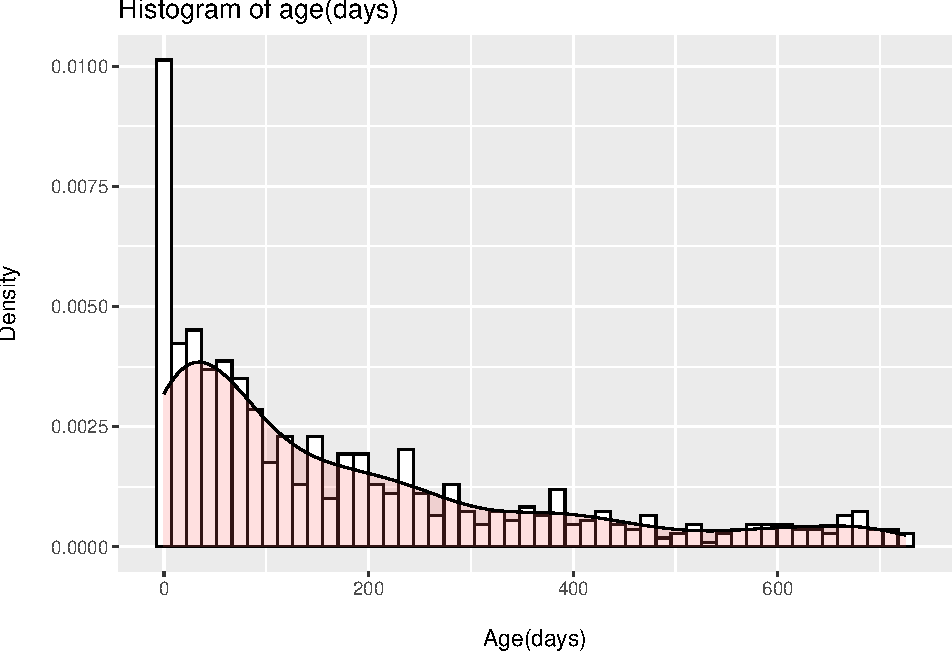
\includegraphics{age_analysis_files/figure-latex/unnamed-chunk-12-1.pdf}

\textbf{Figure 5:} Histogram of age in unit of days (bars) and density
(curve with red area). Here, only cases that evolved into death are
considered.

\begin{Shaded}
\begin{Highlighting}[]
\NormalTok{data\_age2\_death }\SpecialCharTok{\%\textgreater{}\%} 
  \FunctionTok{ggplot}\NormalTok{(}\FunctionTok{aes}\NormalTok{(}\AttributeTok{x =}\NormalTok{ variants,}
             \AttributeTok{y =}\NormalTok{ age\_month,}
             \AttributeTok{fill =}\NormalTok{ variants)) }\SpecialCharTok{+}
  \FunctionTok{geom\_boxplot}\NormalTok{() }\SpecialCharTok{+}
  \FunctionTok{xlab}\NormalTok{(}\StringTok{"}\SpecialCharTok{\textbackslash{}n}\StringTok{Variants"}\NormalTok{) }\SpecialCharTok{+}
  \FunctionTok{ylab}\NormalTok{(}\StringTok{"Age(days)}\SpecialCharTok{\textbackslash{}n}\StringTok{"}\NormalTok{) }\SpecialCharTok{+}
  \FunctionTok{theme}\NormalTok{(}\AttributeTok{legend.position =} \StringTok{"none"}\NormalTok{)}
\end{Highlighting}
\end{Shaded}

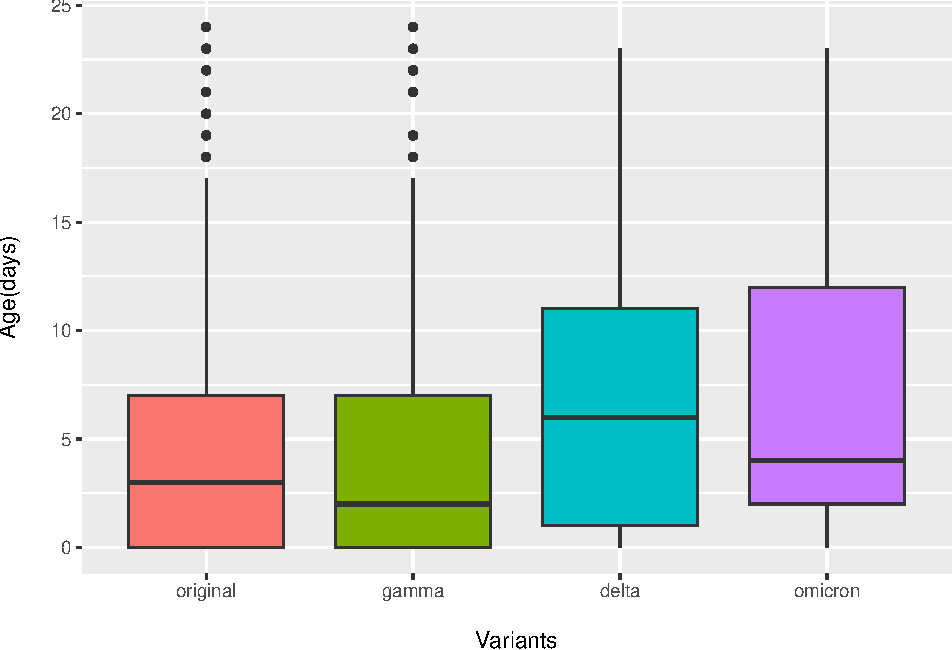
\includegraphics{age_analysis_files/figure-latex/unnamed-chunk-13-1.pdf}

\textbf{Figure 6:} Boxplot of variants by age in a unit of days. Here,
only cases that evolved into death are considered.

\begin{Shaded}
\begin{Highlighting}[]
\FunctionTok{datasummary}\NormalTok{(variants }\SpecialCharTok{\textasciitilde{}}\NormalTok{ idade\_dias}\SpecialCharTok{*}\NormalTok{(n }\SpecialCharTok{+}\NormalTok{ media }\SpecialCharTok{+}\NormalTok{ DP }\SpecialCharTok{+}\NormalTok{ mediana }\SpecialCharTok{+}\NormalTok{ minimo }\SpecialCharTok{+}
\NormalTok{                                   maximo }\SpecialCharTok{+}\NormalTok{ q25 }\SpecialCharTok{+}\NormalTok{ q75 }\SpecialCharTok{+}\NormalTok{ IQR), }
            \AttributeTok{data =}\NormalTok{ data\_age2\_death, }\AttributeTok{output =} \StringTok{\textquotesingle{}markdown\textquotesingle{}}\NormalTok{)}
\end{Highlighting}
\end{Shaded}

\begin{longtable}[]{@{}
  >{\raggedright\arraybackslash}p{(\columnwidth - 18\tabcolsep) * \real{0.1304}}
  >{\raggedleft\arraybackslash}p{(\columnwidth - 18\tabcolsep) * \real{0.0580}}
  >{\raggedleft\arraybackslash}p{(\columnwidth - 18\tabcolsep) * \real{0.1014}}
  >{\raggedleft\arraybackslash}p{(\columnwidth - 18\tabcolsep) * \real{0.1014}}
  >{\raggedleft\arraybackslash}p{(\columnwidth - 18\tabcolsep) * \real{0.1159}}
  >{\raggedleft\arraybackslash}p{(\columnwidth - 18\tabcolsep) * \real{0.1014}}
  >{\raggedleft\arraybackslash}p{(\columnwidth - 18\tabcolsep) * \real{0.1014}}
  >{\raggedleft\arraybackslash}p{(\columnwidth - 18\tabcolsep) * \real{0.0870}}
  >{\raggedleft\arraybackslash}p{(\columnwidth - 18\tabcolsep) * \real{0.1014}}
  >{\raggedleft\arraybackslash}p{(\columnwidth - 18\tabcolsep) * \real{0.1014}}@{}}
\toprule()
\begin{minipage}[b]{\linewidth}\raggedright
variants
\end{minipage} & \begin{minipage}[b]{\linewidth}\raggedleft
n
\end{minipage} & \begin{minipage}[b]{\linewidth}\raggedleft
media
\end{minipage} & \begin{minipage}[b]{\linewidth}\raggedleft
DP
\end{minipage} & \begin{minipage}[b]{\linewidth}\raggedleft
mediana
\end{minipage} & \begin{minipage}[b]{\linewidth}\raggedleft
minimo
\end{minipage} & \begin{minipage}[b]{\linewidth}\raggedleft
maximo
\end{minipage} & \begin{minipage}[b]{\linewidth}\raggedleft
q25
\end{minipage} & \begin{minipage}[b]{\linewidth}\raggedleft
q75
\end{minipage} & \begin{minipage}[b]{\linewidth}\raggedleft
IQR
\end{minipage} \\
\midrule()
\endhead
original & 335 & 156.70 & 177.34 & 92.00 & 0.00 & 725.00 & 19.00 &
222.50 & 203.50 \\
gamma & 217 & 159.51 & 183.56 & 75.00 & 0.00 & 722.00 & 24.00 & 236.00 &
212.00 \\
delta & 41 & 233.07 & 219.76 & 187.00 & 0.00 & 714.00 & 58.00 & 331.00 &
273.00 \\
omicron & 141 & 233.50 & 202.08 & 144.00 & 0.00 & 692.00 & 70.00 &
369.00 & 299.00 \\
\bottomrule()
\end{longtable}

\textbf{Table 5:} Descriptive metrics of age (days) by variants. Here,
only cases that evolved into death are considered.

\hypertarget{agemonths}{%
\subsubsection{Age(months)}\label{agemonths}}

\begin{Shaded}
\begin{Highlighting}[]
\FunctionTok{ggplot}\NormalTok{(data\_age2\_death, }\FunctionTok{aes}\NormalTok{(}\AttributeTok{x =}\NormalTok{ age\_month)) }\SpecialCharTok{+} 
  \FunctionTok{geom\_histogram}\NormalTok{(}\FunctionTok{aes}\NormalTok{(}\AttributeTok{y =} \FunctionTok{after\_stat}\NormalTok{(density)), }
                 \AttributeTok{bins =} \DecValTok{24}\NormalTok{,}
                 \AttributeTok{colour =} \StringTok{"black"}\NormalTok{,}
                 \AttributeTok{fill =} \StringTok{"white"}\NormalTok{) }\SpecialCharTok{+}
  \FunctionTok{geom\_density}\NormalTok{(}\AttributeTok{alpha =}\NormalTok{ .}\DecValTok{2}\NormalTok{, }\AttributeTok{fill =} \StringTok{"\#FF6666"}\NormalTok{) }\SpecialCharTok{+}
  \FunctionTok{labs}\NormalTok{(}\AttributeTok{x =} \StringTok{"}\SpecialCharTok{\textbackslash{}n}\StringTok{Age(month)"}\NormalTok{,}
       \AttributeTok{y =} \StringTok{"Density}\SpecialCharTok{\textbackslash{}n}\StringTok{"}\NormalTok{,}
       \AttributeTok{title =} \StringTok{"Histogram of age(month)"}\NormalTok{)}
\end{Highlighting}
\end{Shaded}

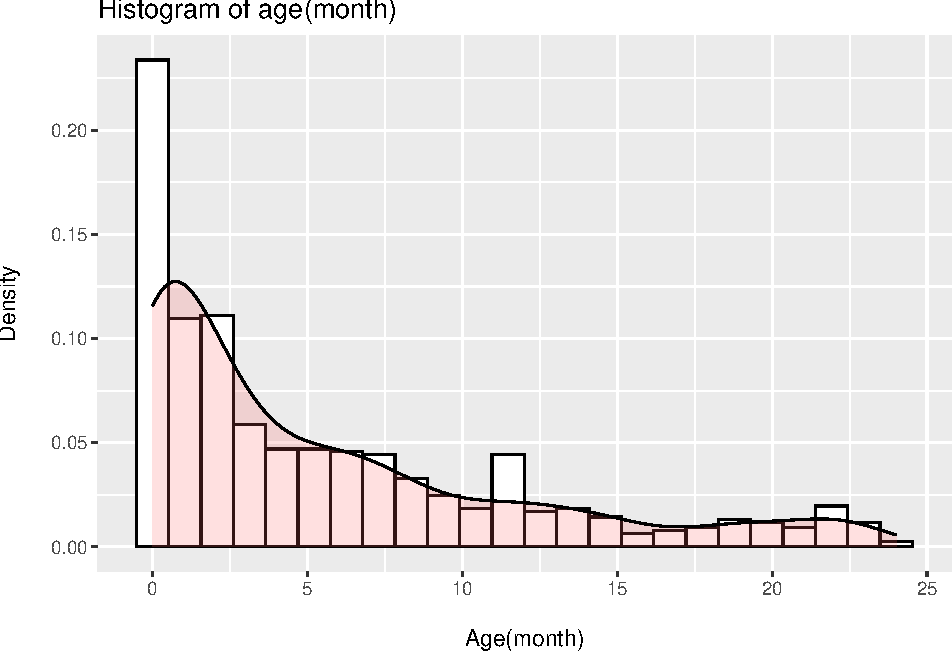
\includegraphics{age_analysis_files/figure-latex/unnamed-chunk-15-1.pdf}

\textbf{Figure 7:} Histogram of age in unit of months (bars) and density
(curve with red area). Here, only cases that evolved into death are
considered.

\begin{Shaded}
\begin{Highlighting}[]
\NormalTok{data\_age2\_death }\SpecialCharTok{\%\textgreater{}\%} 
  \FunctionTok{ggplot}\NormalTok{(}\FunctionTok{aes}\NormalTok{(}\AttributeTok{x =}\NormalTok{ variants,}
             \AttributeTok{y =}\NormalTok{ age\_month,}
             \AttributeTok{fill =}\NormalTok{ variants)) }\SpecialCharTok{+}
  \FunctionTok{geom\_boxplot}\NormalTok{() }\SpecialCharTok{+}
  \FunctionTok{xlab}\NormalTok{(}\StringTok{"}\SpecialCharTok{\textbackslash{}n}\StringTok{Variants"}\NormalTok{) }\SpecialCharTok{+}
  \FunctionTok{ylab}\NormalTok{(}\StringTok{"Age(month)}\SpecialCharTok{\textbackslash{}n}\StringTok{"}\NormalTok{) }\SpecialCharTok{+}
  \FunctionTok{theme}\NormalTok{(}\AttributeTok{legend.position =} \StringTok{"none"}\NormalTok{)}
\end{Highlighting}
\end{Shaded}

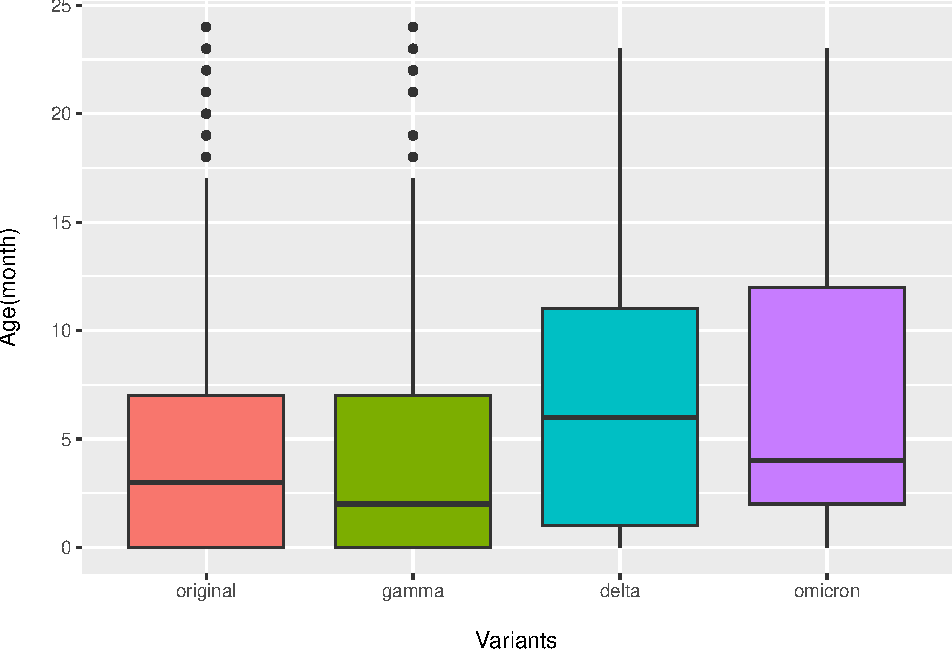
\includegraphics{age_analysis_files/figure-latex/unnamed-chunk-16-1.pdf}

\textbf{Figure 8:} Boxplot of variants by age in a unit of months. Here,
only cases that evolved into death are considered.

\begin{Shaded}
\begin{Highlighting}[]
\FunctionTok{datasummary}\NormalTok{(variants }\SpecialCharTok{\textasciitilde{}}\NormalTok{ age\_month}\SpecialCharTok{*}\NormalTok{(n }\SpecialCharTok{+}\NormalTok{ media }\SpecialCharTok{+}\NormalTok{ DP }\SpecialCharTok{+}\NormalTok{ mediana }\SpecialCharTok{+}\NormalTok{ minimo }\SpecialCharTok{+}
\NormalTok{                                   maximo }\SpecialCharTok{+}\NormalTok{ q25 }\SpecialCharTok{+}\NormalTok{ q75 }\SpecialCharTok{+}\NormalTok{ IQR), }
            \AttributeTok{data =}\NormalTok{ data\_age2\_death, }\AttributeTok{output =} \StringTok{\textquotesingle{}markdown\textquotesingle{}}\NormalTok{)}
\end{Highlighting}
\end{Shaded}

\begin{longtable}[]{@{}
  >{\raggedright\arraybackslash}p{(\columnwidth - 18\tabcolsep) * \real{0.1429}}
  >{\raggedleft\arraybackslash}p{(\columnwidth - 18\tabcolsep) * \real{0.0635}}
  >{\raggedleft\arraybackslash}p{(\columnwidth - 18\tabcolsep) * \real{0.0952}}
  >{\raggedleft\arraybackslash}p{(\columnwidth - 18\tabcolsep) * \real{0.0794}}
  >{\raggedleft\arraybackslash}p{(\columnwidth - 18\tabcolsep) * \real{0.1270}}
  >{\raggedleft\arraybackslash}p{(\columnwidth - 18\tabcolsep) * \real{0.1111}}
  >{\raggedleft\arraybackslash}p{(\columnwidth - 18\tabcolsep) * \real{0.1111}}
  >{\raggedleft\arraybackslash}p{(\columnwidth - 18\tabcolsep) * \real{0.0794}}
  >{\raggedleft\arraybackslash}p{(\columnwidth - 18\tabcolsep) * \real{0.0952}}
  >{\raggedleft\arraybackslash}p{(\columnwidth - 18\tabcolsep) * \real{0.0952}}@{}}
\toprule()
\begin{minipage}[b]{\linewidth}\raggedright
variants
\end{minipage} & \begin{minipage}[b]{\linewidth}\raggedleft
n
\end{minipage} & \begin{minipage}[b]{\linewidth}\raggedleft
media
\end{minipage} & \begin{minipage}[b]{\linewidth}\raggedleft
DP
\end{minipage} & \begin{minipage}[b]{\linewidth}\raggedleft
mediana
\end{minipage} & \begin{minipage}[b]{\linewidth}\raggedleft
minimo
\end{minipage} & \begin{minipage}[b]{\linewidth}\raggedleft
maximo
\end{minipage} & \begin{minipage}[b]{\linewidth}\raggedleft
q25
\end{minipage} & \begin{minipage}[b]{\linewidth}\raggedleft
q75
\end{minipage} & \begin{minipage}[b]{\linewidth}\raggedleft
IQR
\end{minipage} \\
\midrule()
\endhead
original & 335 & 4.81 & 5.86 & 3.00 & 0.00 & 24.00 & 0.00 & 7.00 &
7.00 \\
gamma & 217 & 4.89 & 6.04 & 2.00 & 0.00 & 24.00 & 0.00 & 7.00 & 7.00 \\
delta & 41 & 7.41 & 7.30 & 6.00 & 0.00 & 23.00 & 1.00 & 11.00 & 10.00 \\
omicron & 141 & 7.28 & 6.72 & 4.00 & 0.00 & 23.00 & 2.00 & 12.00 &
10.00 \\
\bottomrule()
\end{longtable}

\textbf{Table 6:} Descriptive metrics of age (months) by variants. Here,
only cases that evolved into death are considered.

\hypertarget{grouped-age-1}{%
\subsection{Grouped age}\label{grouped-age-1}}

\hypertarget{first-case-1}{%
\subsubsection{First case}\label{first-case-1}}

\begin{Shaded}
\begin{Highlighting}[]
\DocumentationTok{\#\#\#\#\#\#\#\# First case \#\#\#\#\#\#\#\#}
\NormalTok{summarytools}\SpecialCharTok{::}\FunctionTok{ctable}\NormalTok{(}
\NormalTok{        data\_age2\_death}\SpecialCharTok{$}\NormalTok{age\_months\_firstcase,}
\NormalTok{        data\_age2\_death}\SpecialCharTok{$}\NormalTok{variants,}
        \AttributeTok{prop =} \StringTok{"c"}\NormalTok{,}
        \AttributeTok{headings =} \FunctionTok{st\_options}\NormalTok{(}\StringTok{"headings"}\NormalTok{),}
        \AttributeTok{display.labels =} \FunctionTok{st\_options}\NormalTok{(}\StringTok{"display.labels"}\NormalTok{),}
        \AttributeTok{useNA =} \StringTok{"ifany"}\NormalTok{,}
        \AttributeTok{OR =} \ConstantTok{TRUE}\NormalTok{,}
        \AttributeTok{chisq =} \ConstantTok{TRUE}
\NormalTok{      )}
\end{Highlighting}
\end{Shaded}

\begin{longtable}[]{@{}lrrrrrr@{}}
\toprule()
\endhead
& variants & original & gamma & delta & omicron & Total \\
age\_months\_firstcase & & & & & & \\
1 month & & 105 ( 31.3\%) & 61 ( 28.1\%) & 5 ( 12.2\%) & 11 ( 7.8\%) &
182 ( 24.8\%) \\
between 1 and 6 months & & 121 ( 36.1\%) & 81 ( 37.3\%) & 15 ( 36.6\%) &
66 ( 46.8\%) & 283 ( 38.6\%) \\
between 6 and 12 months & & 63 ( 18.8\%) & 43 ( 19.8\%) & 12 ( 29.3\%) &
28 ( 19.9\%) & 146 ( 19.9\%) \\
more than 12 months & & 46 ( 13.7\%) & 32 ( 14.7\%) & 9 ( 22.0\%) & 36 (
25.5\%) & 123 ( 16.8\%) \\
Total & & 335 (100.0\%) & 217 (100.0\%) & 41 (100.0\%) & 141 (100.0\%) &
734 (100.0\%) \\
\bottomrule()
\end{longtable}

\begin{longtable}[]{@{}
  >{\centering\arraybackslash}p{(\columnwidth - 4\tabcolsep) * \real{0.1944}}
  >{\centering\arraybackslash}p{(\columnwidth - 4\tabcolsep) * \real{0.0694}}
  >{\centering\arraybackslash}p{(\columnwidth - 4\tabcolsep) * \real{0.1389}}@{}}
\toprule()
\begin{minipage}[b]{\linewidth}\centering
Chi.squared
\end{minipage} & \begin{minipage}[b]{\linewidth}\centering
df
\end{minipage} & \begin{minipage}[b]{\linewidth}\centering
p.value
\end{minipage} \\
\midrule()
\endhead
40.4386 & 9 & 0 \\
\bottomrule()
\end{longtable}

\textbf{Table 7:} Age(months) versus variants, where age is grouped as:
\textless= 30 days (1 month); 31 days \textbar- 180 days (between 1 and
6 months); 181 days \textbar- 365 days (between 6 and 12 months);
\textgreater= 366 days (more than 12 months). Here, only cases that
evolved into death are considered.

\hypertarget{second-case-1}{%
\subsubsection{Second case}\label{second-case-1}}

\begin{Shaded}
\begin{Highlighting}[]
\DocumentationTok{\#\#\#\#\#\#\#\# Second case \#\#\#\#\#\#\#\#}
\NormalTok{summarytools}\SpecialCharTok{::}\FunctionTok{ctable}\NormalTok{(}
\NormalTok{        data\_age2\_death}\SpecialCharTok{$}\NormalTok{age\_months\_secondcase,}
\NormalTok{        data\_age2\_death}\SpecialCharTok{$}\NormalTok{variants,}
        \AttributeTok{prop =} \StringTok{"c"}\NormalTok{,}
        \AttributeTok{headings =} \FunctionTok{st\_options}\NormalTok{(}\StringTok{"headings"}\NormalTok{),}
        \AttributeTok{display.labels =} \FunctionTok{st\_options}\NormalTok{(}\StringTok{"display.labels"}\NormalTok{),}
        \AttributeTok{useNA =} \StringTok{"ifany"}\NormalTok{,}
        \AttributeTok{OR =} \ConstantTok{TRUE}\NormalTok{,}
        \AttributeTok{chisq =} \ConstantTok{TRUE}
\NormalTok{      )}
\end{Highlighting}
\end{Shaded}

\begin{longtable}[]{@{}lrrrrrr@{}}
\toprule()
\endhead
& variants & original & gamma & delta & omicron & Total \\
age\_months\_secondcase & & & & & & \\
1 month & & 105 ( 31.3\%) & 61 ( 28.1\%) & 5 ( 12.2\%) & 11 ( 7.8\%) &
182 ( 24.8\%) \\
between 1 and 6 months & & 121 ( 36.1\%) & 81 ( 37.3\%) & 15 ( 36.6\%) &
66 ( 46.8\%) & 283 ( 38.6\%) \\
between 6 and 12 months & & 63 ( 18.8\%) & 43 ( 19.8\%) & 12 ( 29.3\%) &
28 ( 19.9\%) & 146 ( 19.9\%) \\
between 12 and 18 months & & 27 ( 8.1\%) & 18 ( 8.3\%) & 2 ( 4.9\%) & 18
( 12.8\%) & 65 ( 8.9\%) \\
more than 18 months & & 19 ( 5.7\%) & 14 ( 6.5\%) & 7 ( 17.1\%) & 18 (
12.8\%) & 58 ( 7.9\%) \\
Total & & 335 (100.0\%) & 217 (100.0\%) & 41 (100.0\%) & 141 (100.0\%) &
734 (100.0\%) \\
\bottomrule()
\end{longtable}

\begin{longtable}[]{@{}
  >{\centering\arraybackslash}p{(\columnwidth - 4\tabcolsep) * \real{0.1944}}
  >{\centering\arraybackslash}p{(\columnwidth - 4\tabcolsep) * \real{0.0694}}
  >{\centering\arraybackslash}p{(\columnwidth - 4\tabcolsep) * \real{0.1389}}@{}}
\toprule()
\begin{minipage}[b]{\linewidth}\centering
Chi.squared
\end{minipage} & \begin{minipage}[b]{\linewidth}\centering
df
\end{minipage} & \begin{minipage}[b]{\linewidth}\centering
p.value
\end{minipage} \\
\midrule()
\endhead
45.7022 & 12 & 0 \\
\bottomrule()
\end{longtable}

\textbf{Table 8:} Age(months) versus variants, where age is grouped as:
\textless= 30 days (1 month); 31 days \textbar- 180 days (between 1 and
6 months); 181 days \textbar- 365 days (between 6 and 12 months); 366
days \textbar- 545 days (between 12 and 18 months); \textgreater= 546
days (more than 18 months). Here, only cases that evolved into death are
considered.

\end{document}
